\chapter{\emph{\arr Project}: Torchelie}

\section{Motivations}

Back in Montréal, working for JSALT2019, I wanted to gather all the deep learning related code I wrote so far for my job and thesis. The initial motivation to realize this project was clear: while deep learning code is often short to write, it is also extremely easy to get wrong, and even harder to diagnose and debug. In standard software engineering, most mistakes end up crashing the app or raising exceptions, making them obvious to uncover. In deep learning, they cripple the results, often in very subtle ways.

Besides, many code bases would share common patterns: training and testing loops, alternating training for G and D in GANs, measuring accuracy, layers or blocks, etc. In most public code, the training code is often made of raw for-loop instrumented with many ifs, and as the need to monitor new quantities grow, the code gets harder to maintain and error prone. As we try new incremental ideas, the ifs switches grow out of hand, readability suffers, and more bugs arise.

Torchélie is a software engineering take to tackle this problem and provide tools to build both experiments and production-ready code that is fast to write and easy to maintain, from battle tested building blocks.

\section{Design Principles}

Torchélie follows design patterns thought to be adapted to the task at hand. Torchélie follows few design principles:

\begin{enumerate}
    \item \textbf{Independent} As much as possible, features must be independent and one must be able to use exactly the feature they need without difficulty. For instance, one must be able to use a layer or a model in their project and use them as much as possible as Pytorch components in their Pytorch project. One might be able to train a vanilla Pytorch model with a training loop from Torchélie without any adaptation.
    
    \item \textbf{Compositionality} Features are built by composing small and independent building blocks. All blocks must do one thing and do it well. Greater components must be designed by combining smaller components and keep the logic simple. The user should be able to easily write their own components and easily compose them to the set of feature that is looked for. For instance, it must be easy to write a new type of layer and use it in the provided models with minimal pain; to write a new metric to integrate in the training loop; to write a new training logic code; etc.
    
    \item \textbf{Build standard and modify} Trying to build models, training recipes, layers, with options for customization inside the object constructors leads to two kind of major issues. First, despite the best efforts, it is very hard to know what the user will want to control. Second, the code either lacks customizability or becomes unmaintainable as one adds switches and parameters. Moreover, each layer option must be ported as well to the model's options, and the parameters and switches grow totally out of hand. In training code, this happens the same way as one might want to change a loss function, add one, etc. Instead, we should provide simple ways to build standard components, and give editing features. Instead of building customized, it is hypothesized that thinking in terms of deltas from the standard blocks scales better: the construction code remain simple and straightforward as it builds just one standard thing, and the edition functions remain external and self contained.
    
    Training code should follow the same guidelines. For instance, complex losses such as the Pix2pixHD loss should be simple but composable so that a user can easily add, remove, change or replace one term.
    
    Incremental changes are the bread and butter of the deep learning practitioner as we try changes from a standard algorithm and evaluate their performance; let's keep these deltas expressed as deltas in the code as well.
\end{enumerate}

\subsection{Models}

Torchélie provide many architectures, that are yet to be pretrained. It provides many resnet variants and GANs architectures such as Pix2pix or StyleGAN2.

It becomes straightforward to write code in Torchelie style. The model or block is implemented in its most basic, go-to form. Derivative models are implemented in terms of transforms from those basic blocks.

For instance, a standard residual bottleneck block from ResNet-50 is written in its most standard and least parametric possible way, just making sure every module and submodule is conveniently named:

\begin{lstlisting}[language=Python, caption=A ResBlock in Torchelie]
class ResBlockBottleneck(nn.Module):
    """
    A Residual Block. Skip connection will be added if the number of input and
    output channels don't match or stride > 1 is used.
    Args:
        in_ch (int): input channels
        out_ch (int): output channels
        stride (int): stride
    """

    def __init__(self,
                 in_channels: int,
                 out_channels: int,
                 stride: int = 1) -> None:
        super(ResBlockBottleneck, self).__init__()
        self.in_channels = in_channels
        self.out_channels = out_channels
        self.stride = stride

        self.pre = CondSeq()

        self.wide(divisor=4)

        self.shortcut = _make_resnet_shortcut(in_channels, out_channels, stride)

        self.post = CondSeq()
        self.post.relu = nn.ReLU(True)

    def wide(self, divisor: int = 2) -> 'ResBlockBottleneck':
        in_ch = self.in_channels
        out_ch = self.out_channels
        mid = out_ch // divisor
        stride = self.stride

        self.branch = CondSeq(
            collections.OrderedDict([
                ('conv1', kaiming(Conv1x1(in_ch, mid, bias=False))),
                ('bn1', constant_init(nn.BatchNorm2d(mid), 1)),
                ('relu', nn.ReLU(True)),
                ('conv2', kaiming(Conv3x3(mid, mid, stride=stride,
                                          bias=False))),
                ('bn2', constant_init(nn.BatchNorm2d(mid), 1)),
                ('relu2', nn.ReLU(True)),
                ('conv3', kaiming(Conv1x1(mid, out_ch, bias=False))),
                ('bn3', constant_init(nn.BatchNorm2d(out_ch), 0)),
            ]))
        return self

    def forward(self,
                x: torch.Tensor,
                z: Optional[torch.Tensor] = None) -> torch.Tensor:
        if z is not None:
            self.condition(z)

        x = self.pre(x)
        x = self.branch(x).add_(self.shortcut(x))
        return self.post(x)
\end{lstlisting}

This already allows to transform a residual block into its Wide ResNet \cite{wrn} counterpart. Similarly, we can write functions that remove batchnorms:


\begin{lstlisting}[language=Python, caption=A ResBlock in Torchelie]
    def remove_batchnorm(self) -> 'ResBlockBottleneck':
        remove_batchnorm(self.branch)
        remove_batchnorm(self.shortcut)
        assert isinstance(self.branch.conv3, nn.Conv2d)
        constant_init(self.branch.conv3, 0)

        return self
\end{lstlisting}

Or adds Squeeze-And-Excite blocks \cite{squeezeexcitation}

\begin{lstlisting}[language=Python, caption=Add Squeeze-And-Excite module]
    def use_se(self) -> 'ResBlockBottleneck':
        self.branch.add_module('se', SEBlock(self.out_channels))
        return self
\end{lstlisting}

Change the convs to ResNeXt \cite{resnext}:

\begin{lstlisting}[language=Python, caption=ResNeXt]
    def resnext(self) -> 'ResBlockBottleneck':
        self.wide(divisor=2)
        c = self.branch.conv2
        assert isinstance(c, nn.Conv2d)
        self.branch.conv2 = kaiming(
            nn.Conv2d(c.in_channels,
                      c.out_channels,
                      kernel_size=3,
                      padding=1,
                      stride=self.stride,
                      bias=c.bias is not None,
                      groups=32))
        return self
\end{lstlisting}

\subsection{Algorithms}

We can also demonstrate with concrete code how those design guidelines apply to algorithms implementation. Central to this is the Algorithm class. It is a glorified list of named functions. Those functions are called in order when calling the algorithm. The names allow to easily manipulate the list in order to replace or remove existing functions, or insert new ones. That way, algorithms can be described in atomic step that can be incrementally manipulated to grow more sophisticated versions or forked variants.

Let's see the implementation for Pix2Pix. Pix2Pix is a conditional GAN that concatenates the source and target image to the discriminator. The G pass is made in two steps: generate some fakes and compute the loss; then backpropagate. The D pass is performed in two steps as well: generate some fakes; then compute and backpropagate real and fake loss for D. Those steps could and maybe should be made even more atomic.

\begin{lstlisting}[language=Python, caption=ConcatConditionalGAN. The implementation details are removed in order to focus on the design principles.]
class ConcatConditionalGANLoss:

    def __init__(self, G: nn.Module, D: nn.Module) -> None:
        self.G = G
        self.D = D
        self.gan_loss = tch.loss.gan.standard

        G_alg = Algorithm()

        @G_alg.add_step('adversarial')
        def G_adv_pass(env, src, dst):
            # Generate some fakes, compute the discriminator loss

        @G_alg.add_step('backward')
        def backward(env, src, dst):
            # backward the discriminator loss

        self.G_alg = G_alg

        D_alg = Algorithm()

        @D_alg.add_step('gen_fakes')
        def gen_fakes(env, src, dst):
            # Generate fake images

        @D_alg.add_step('adversarial')
        def D_fake(env, src, dst):
            # Compute the discriminator loss for real and fake
            # samples. Backpropagate. Return some metrics

        self.D_alg = D_alg

    def G_step(self, src: torch.Tensor, dst: torch.Tensor) -> dict:
        return self.G_alg(src, dst)

    def D_step(self, src: torch.Tensor, dst: torch.Tensor) -> dict:
        return self.D_alg(src, dst)
\end{lstlisting}

A variant could use the R1 regularizer \cite{R1}. This could be achieved by adding a gradient penalty computation before performing the backpropagation on D:

\begin{lstlisting}[language=Python, caption=ConcatConditionalGAN with R1 regularizer]
    def use_r1(self, r1_gamma):
        self.gan_loss = tch.loss.gan.standard
        gradient_penalty = GradientPenalty(r1_gamma)

        @self.D_alg.insert_before('adversarial', 'D_r1')
        def D_r1(env, src, dst):
            with self.D.no_sync():
                g_norm = gradient_penalty(self.D, env['real_pair'] * 2 - 1,
                                          env['fake_pair'] * 2 - 1)
            return {'g_norm': g_norm}
\end{lstlisting}

Pix2Pix extends the standard conditional GAN with a L1 loss between the generated picture and the actual target picture. Inheritance can achieve this.

\begin{lstlisting}[language=Python, caption=Pix2Pix from ConcatConditionalGAN]
class Pix2PixLoss(ConcatConditionalGANLoss):

    def __init__(self, G: nn.Module, D: nn.Module, l1_gain: float) -> None:
        super().__init__(G, D)
        self.l1_gain = l1_gain

        @self.G_alg.insert_after('adversarial', 'l1')
        def G_l1_pass(env, src, dst):
            loss = self.l1_gain * F.l1_loss(env['out'], dst)
            env['loss'] += loss
            return {'l1_loss': loss.item()}
\end{lstlisting}

Instead, Pix2PixHD is a derivative work that mostly incorporates a feature matching loss to the standard conditional GAN setting and switches to the Least-Squares GAN loss they find more stable.

\begin{lstlisting}[language=Python, caption=Pix2PixHD]
class Pix2PixHDLoss(ConcatConditionalGANLoss):

    def __init__(self, G: nn.Module, D: nn.Module, l1_gain: float):
        super().__init__(G, D)
        self.gan_loss = tch.loss.gan.ls
        self.l1_gain = l1_gain

        D_with_acts = tnn.WithSavedActivations(D.module)

        @self.G_alg.insert_before('adversarial', 'extract_features')
        def G_features(env, src, dst):
            # Generate fake samples, compute D's activations and its final
            # predicted probability

        @self.G_alg.insert_after('extract_features', 'feature_matching')
        def G_featmatch(env, src, dst):
            # Compute the feature matching loss

        @self.G_alg.override_step('adversarial')
        def G_adv(env, src, dst):
            # add the actual adversarial loss
\end{lstlisting}

The incremental nature of the work becomes totally apparent and fully manipulable. Easy experiments can be conducted if one wishes to remove, replace, or add elements to the feature matching loss for instance, or add a VGG loss that became popular later.

\section{Provided Features}

\subsection{Models}


Torchélie provides models, but only a few are pretrained due to lack of compute resources. It provides code for a wide variety of ResNets \cite{resnet} (upgraded ResNets \cite{resnettricks}, with SE blocks \cite{squeezeexcitation}, wides \cite{wrn}, with preactivation \cite{preact}, ResNeXt \cite{resnext}), EfficientNets \cite{efficientnet}, GANs (StyleGAN2 \cite{stylegan2}, AutoGAN \cite{autogan}, Patch discriminators \cite{pix2pix}, Spectral Normalization GANs \cite{SNGAN}). Vision Transformers are the next models to be integrated.

Contrarily to all general purpose known libraries to date, Torchélie would be the first one to propose models pretrained on other datasets than ImageNet, by embedding, in a near future, models pretrained on face recognition and detection tasks.

\subsection{Recipes}

\begin{figure}[h]
    \centering
    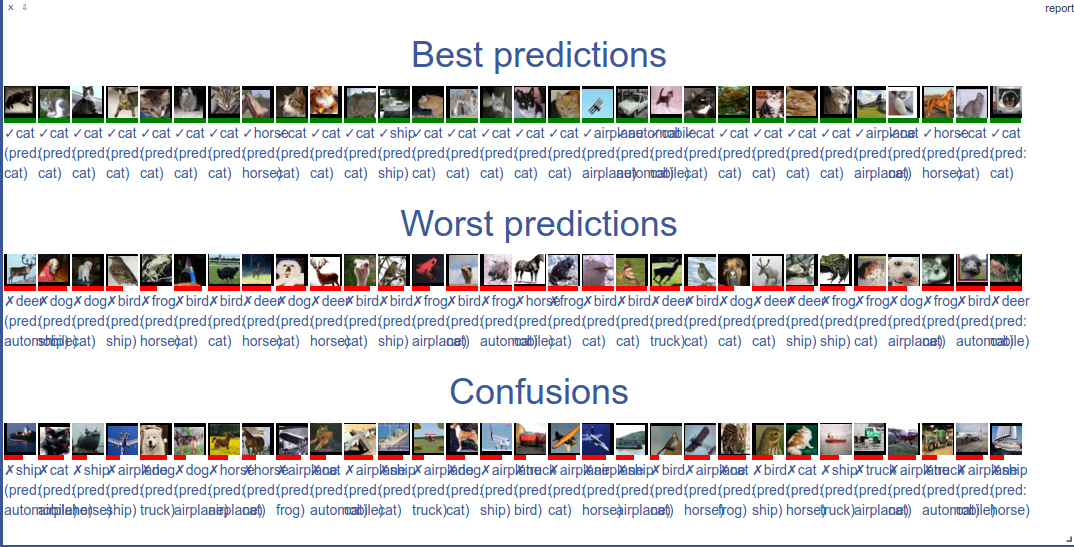
\includegraphics[width=\columnwidth]{90-files/classifreport.png}
    \caption{The ClassificationInspector allows to see live the performance of the classifier. It reports the samples that are provide the best, worst, and most confused answers from the classifier. The bar below the images is green when the prediction is correct, red otherwise; the width reflects the confidence score of the prediction. This allows eyeballing the datasets, strengths and weaknesses of the model, and build intuition.}
    \label{fig:classifreport}
\end{figure}

\begin{figure}[h]
    \centering
    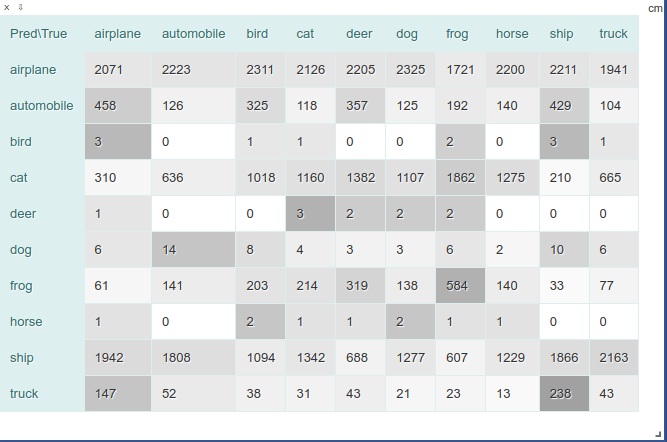
\includegraphics[width=\columnwidth]{90-files/confmatrix.png}
    \caption{Live confusion matrix provided automatically when the number of classes is not too big to make it unreadable (less than 25 classes).}
    \label{fig:confmatrix}
\end{figure}

\begin{figure}
    \centering
    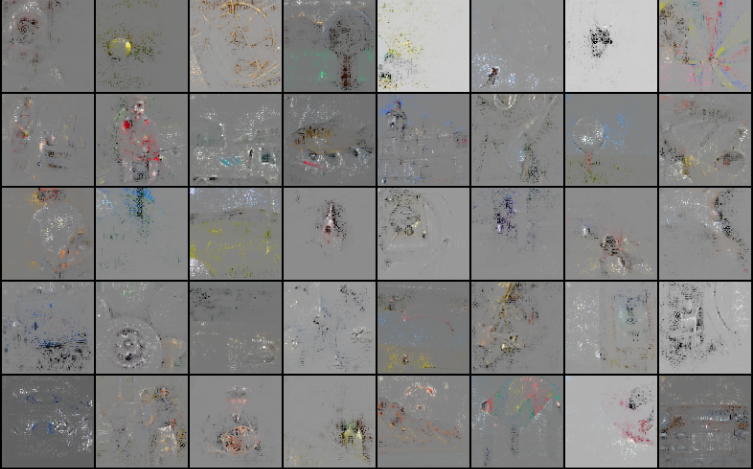
\includegraphics[width=\columnwidth]{90-files/gradients.png}
    \caption{Gradient of the loss wrt the input on the current batch. The per-pixel norm of the gradient weighs each pixel's intensity. This helps figuring out what the model looks at in the picture in order to make its predictions}
    \label{fig:gradients}
\end{figure}

Recipes are provided algorithms that are often usable with a simple command line. Torchelie provides simple image classification recipes, as well as less common feature visualization, GAN training, Deep Dream.

Those recipes are also usable as python API, and can be used with many of the callbacks that are provided. They allow to track many metrics, perform sanity checks with live visualization (Figure \ref{fig:classifreport} for the classification report, \ref{fig:confmatrix} for the confusion matrix, \ref{fig:gradients} for the gradients).

\section{Conclusion}


Torchélie is an invaluable tool for both my academic and industrial work. There is a virtuous double-way feedback loop at play: Torchélie helps my works and its use allows me to figure out the tools and designs needed in the library. This symbiotic flow also allows to proof test the code and ensure its correctness and performance.

The use case for Torchélie could be questioned now that other libraries such as timm \cite{timm}, fastai \cite{fastai}, Ignite \cite{ignite}, or PyTorch-Lightning are getting traction.

\begin{enumerate}
    \item timm provides a very large quantity of models, most of which are also pretrained on ImageNet. However, its scope remains focused on training image classifiers.
    \item fastai is closer in its scope to Torchélie. Fastai has some different design opinion that makes it feel like learning an entirely novel library. Fastai mostly sits on top of Pytorch rather than extending it horizontally.
    \item Finally, Ignite and PyTorch-Lightning are source of inspiration and close to what I envision. Torchélie tries to be more task oriented at the cost of flexibility, and fit my needs better.
\end{enumerate}

In the long run, the broad scope of Torchélie does not seem sustainable and should either narrow its scope or integrate at least parts of the aforementioned libraries in order to remain relevant with a sustainable work load. The field is advancing faster every day and more means are needed today to keep up with the pace than when it started.

